\documentclass[]{article}
\usepackage{amssymb,latexsym,amsmath}     % Standard packages
\usepackage[pdftex]{graphicx}
\usepackage{indentfirst}
\renewcommand{\baselinestretch}{1.05} 

\addtolength{\textwidth}{1.0in}
\addtolength{\textheight}{1.00in}
\addtolength{\evensidemargin}{-0.75in}
\addtolength{\oddsidemargin}{-0.75in}
\addtolength{\topmargin}{-.50in}
\usepackage[lf]{venturis}
% \usepackage[T1]{fontenc}
% \usepackage{newtxtext,newtxmath}
% \renewcommand{\familydefault}{\sfdefault}  % sans-serif!

\usepackage{fancyhdr}
\renewcommand\headrule{}
\pagestyle{fancy}
\fancyhf{}
\lhead{Non-digital Prototype\\
CS/INFO 3152}
\rhead{\resizebox{0.75in}{!}{
\includegraphics{img/logo_team.jpg}}}
\rfoot{\thepage}

\begin{document}

\title{Non-digital Prototype}
\author{Team \emph{wut} - Kylar Henderson, Charles Tark,\\ 
Gagik Hakobyan, Julia Cole, Andrew Halpern, Austin Liu}
\date{} % removed date
\maketitle

\section*{Game Rules}

The players' objective is to navigate the map to get the character to
the end tile. The bar at the top represents what action the players
must take on each beat of the song. If the rhythm ticker is on a space
with no action, the players are free to perform any action on the
gameboard except standing idle. If the rhythm ticker is hovered over
an action icon on the rhythm bar the players must take that action on
the map to move onto the next action. If players miss a specified
action, the players lose and restart from the starting tile. A picture
of a sword indicates players must land on the same tile as an enemy to
attack and defeat that enemy. A picture of the blue circle means that
the players must land on the blue circle which completes the level.\\

The players have three actions they can take. First, they can move one
tile in any cardinal direction. This action is available on all three
levels. Second, players can jump. This allows them to move two tiles
in any one cardinal direction. This action is only allowed on the
medium and hard levels. Finally, the players can freeze
enemies. Players are only allowed to freeze once per level and this
action is only allowed on the hard level. When the players use freeze,
all enemies on the board stop moving for the next three players'
actions and then resume movement as normal.

\pagebreak
\section*{Pictures}


\begin{figure}[!htb]
\begin{center}

\resizebox{3.0in}{!}{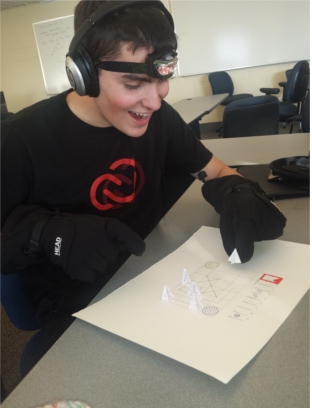
\includegraphics{img/andrew.jpg}}
\end{center}
\caption{Andrew enjoying our non-digital prototype \label{andrew}}
\end{figure}


\begin{figure}[!htb]
\begin{center}
\leavevmode
\resizebox{4.0in}{!}{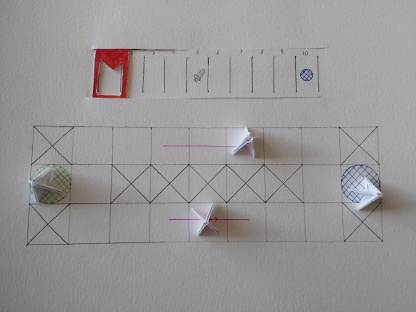
\includegraphics{img/level_easy.jpg}}
\end{center}
\caption{Easy Level \label{level_easy}}
\end{figure}


\begin{figure}[!htb]
\begin{center}
\leavevmode
\resizebox{4.0in}{!}{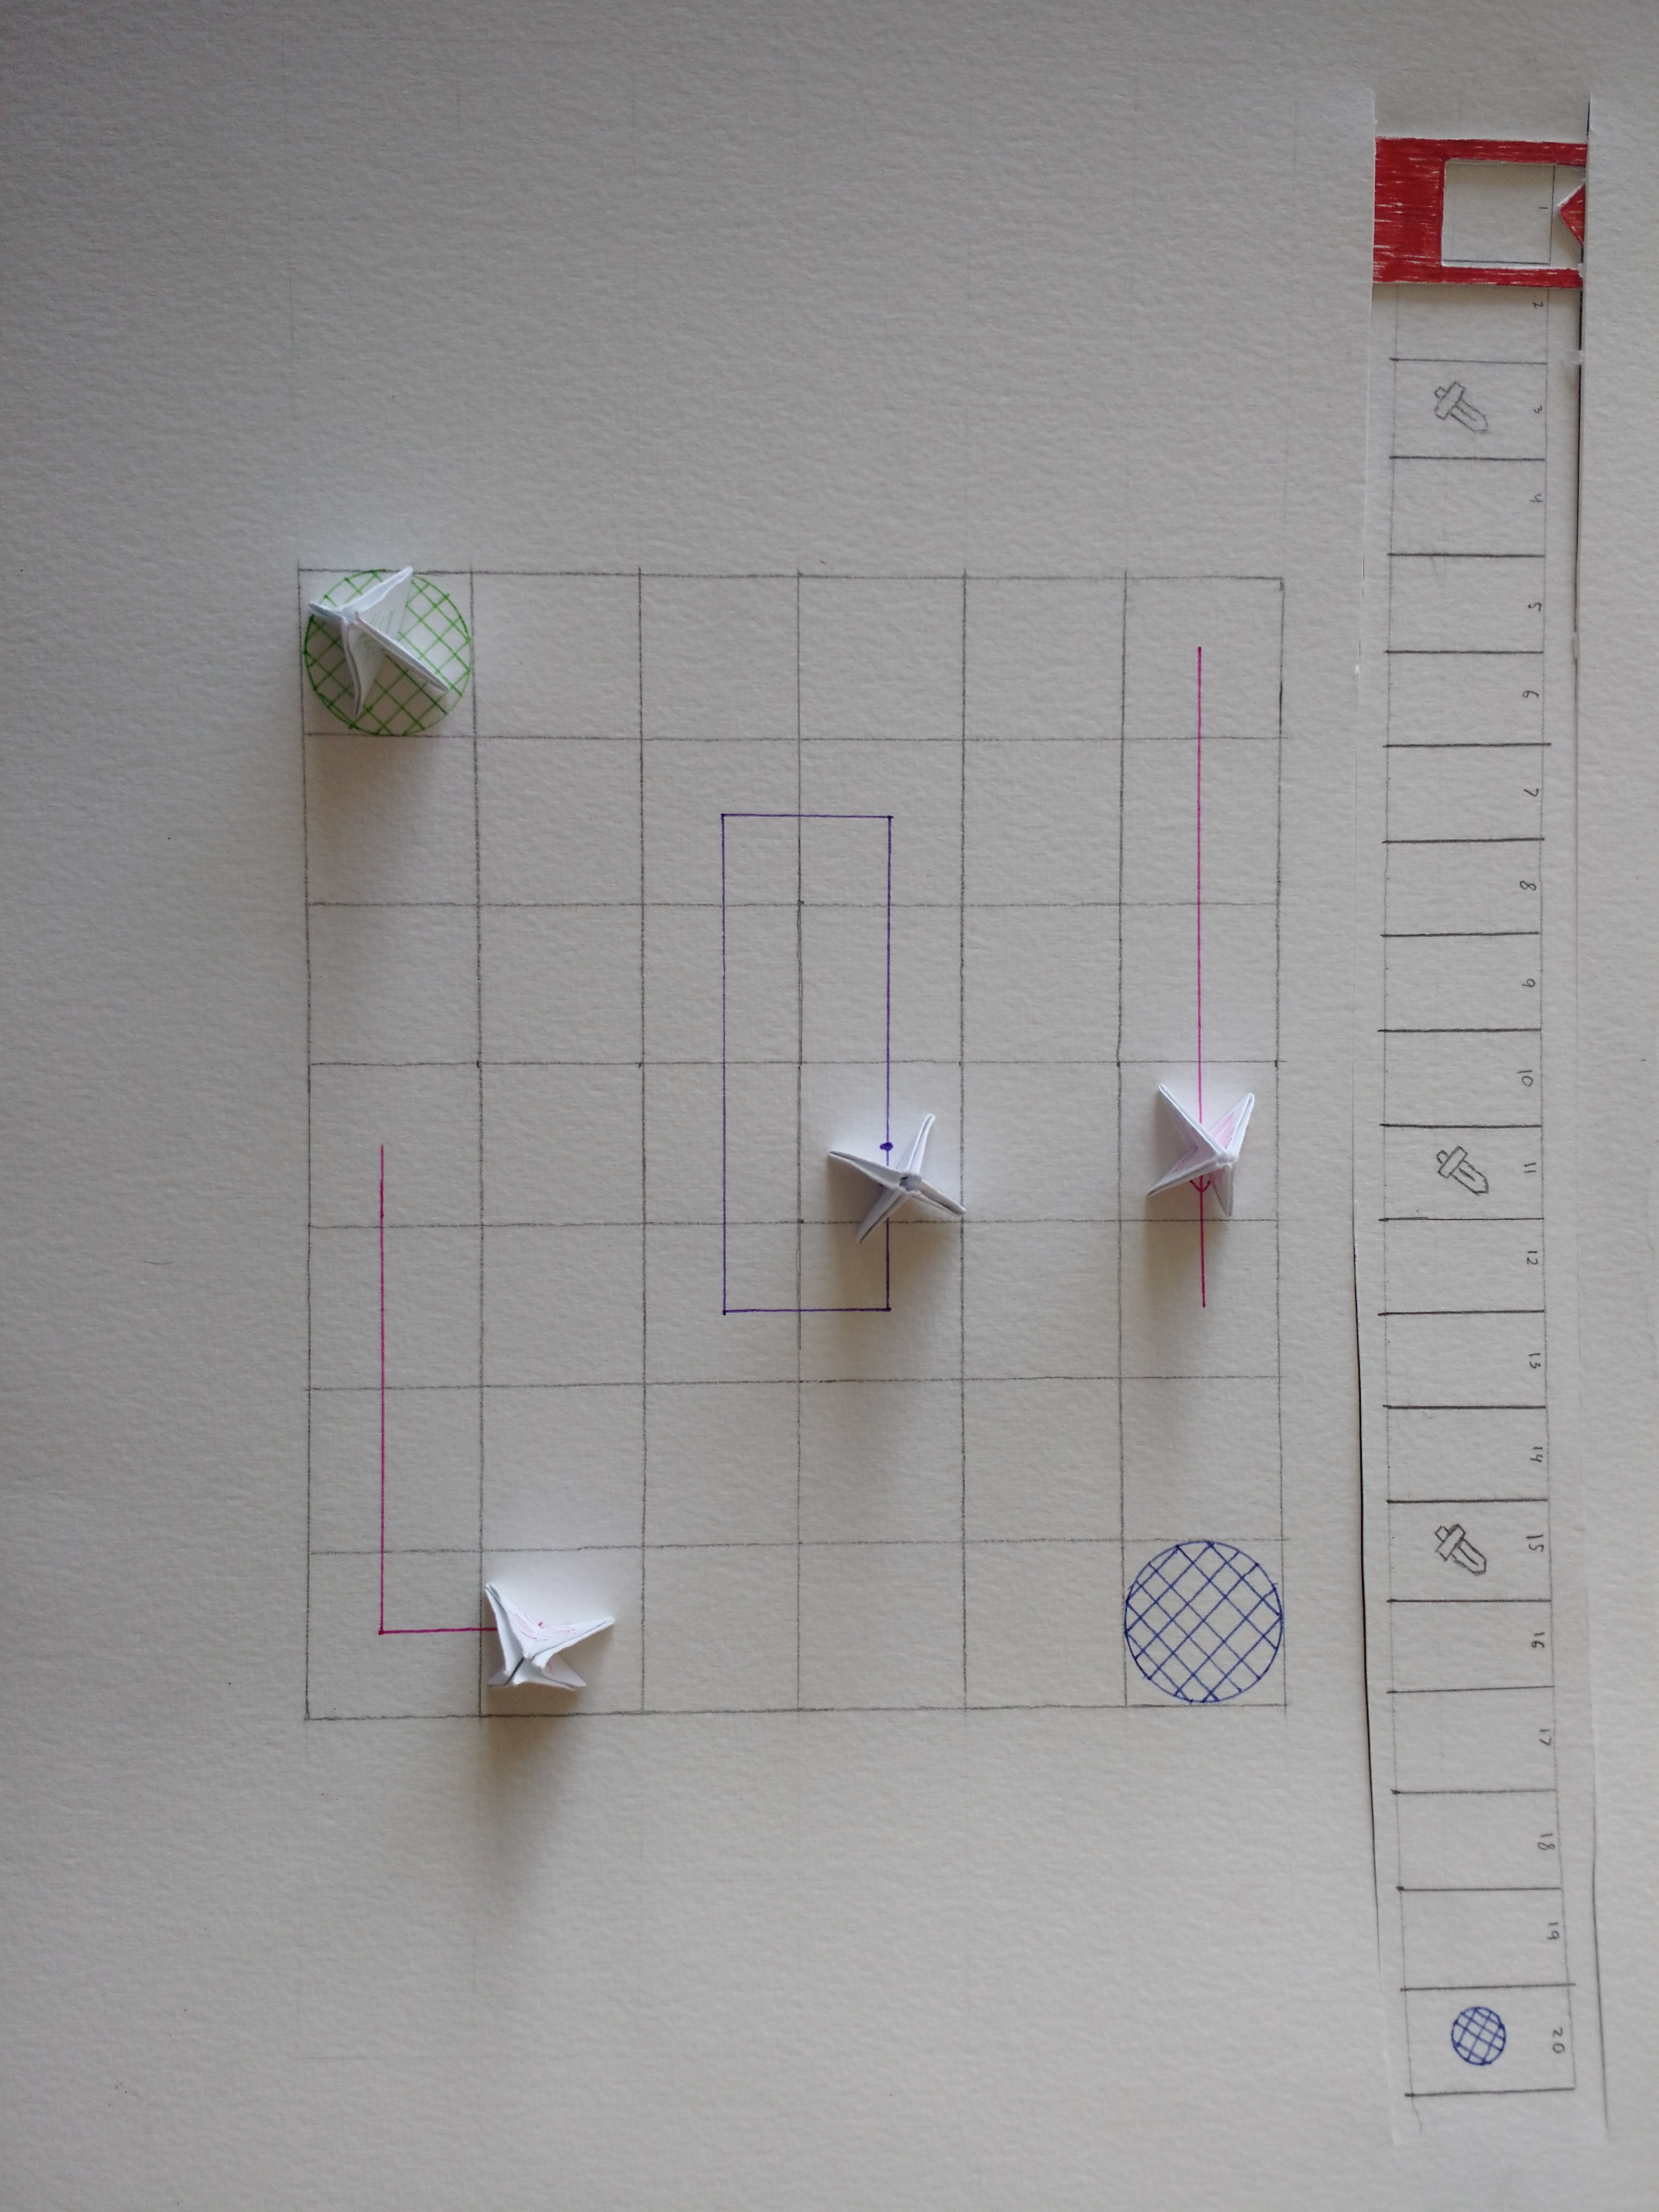
\includegraphics{img/level_medium.jpg}}
\end{center}
\caption{Medium Level \label{level_medium}}
\end{figure}


\begin{figure}[!htb]
\begin{center}
\leavevmode
\resizebox{4.0in}{!}{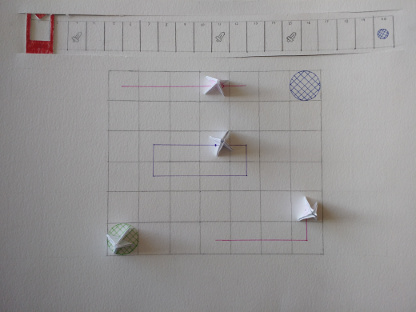
\includegraphics{img/level_hard.jpg}}
\end{center}
\caption{Hard Level \label{level_hard}}
\end{figure}




\end{document}
